\documentclass[11pt,a4paper]{article}
\usepackage[utf8]{inputenc}
\usepackage[margin=0.85in]{geometry}
\usepackage{amsmath,amssymb,amsthm}
\usepackage{xcolor}
\usepackage{tcolorbox}
\usepackage{tikz}
\usetikzlibrary{shapes,arrows,positioning,calc,decorations.pathreplacing,patterns}
\usepackage{booktabs}
\usepackage{array}
\usepackage{fancyhdr}
\usepackage{hyperref}
\usepackage{microtype}

% Color Palette Definitions
\definecolor{primarynavy}{RGB}{26, 54, 93}       % #1A365D - Deep Navy
\definecolor{secondaryteal}{RGB}{13, 148, 136}   % #0D9488 - Teal Accent
\definecolor{darkslate}{RGB}{45, 55, 72}        % #2D3748 - Body Text
\definecolor{lightbg}{RGB}{247, 250, 252}        % #F7FAFC - Soft Background
\definecolor{accentblue}{RGB}{49, 130, 206}      % #3182CE - Bright Blue
\definecolor{warmgold}{RGB}{214, 158, 46}        % #D69E2E - Gold Highlight
\definecolor{crimsonred}{RGB}{229, 62, 62}       % #E53E3E - Crimson Alert

\hypersetup{
    colorlinks=true,
    linkcolor=primarynavy,
    citecolor=secondaryteal,
    urlcolor=accentblue,
    pdftitle={Metric Spaces: New Lectures on Open and Closed Sets, Closures, Interiors, and Subspaces},
    pdfauthor={Class Notes}
}

% Page Setup
\pagestyle{fancy}
\fancyhf{}
\fancyhead[L]{\small \textbf{\color{primarynavy}Metric Spaces: Advanced Topics (MATMJ53)}}
\fancyhead[R]{\small \textbf{\color{secondaryteal}Lectures by AP Sir}}
\fancyfoot[L]{\small \textcolor{primarynavy}{\href{https://www.sciqb.com}{\textbf{www.sciqb.com}}}}
\fancyfoot[C]{\thepage}
\fancyfoot[R]{\small \textcolor{secondaryteal}{\href{https://www.sciqb.com}{\textbf{SCIQB Platform}}}}
\renewcommand{\headrulewidth}{0.6pt}
\renewcommand{\footrulewidth}{0.4pt}

% Custom TColorBox Environments
\newtcolorbox{defbox}[1]{
    colback=lightbg,
    colframe=primarynavy,
    fonttitle=\bfseries\color{white},
    title={#1},
    boxrule=1pt,
    top=3mm, bottom=3mm, left=4mm, right=4mm
}

\newtcolorbox{formulabox}[1]{
    colback=secondaryteal!8!white,
    colframe=secondaryteal,
    fonttitle=\bfseries\color{white},
    title={#1},
    boxrule=1pt,
    top=3mm, bottom=3mm, left=4mm, right=4mm
}

\newtcolorbox{exbox}[1]{
    colback=white,
    colframe=accentblue,
    fonttitle=\bfseries\color{white},
    title={#1},
    boxrule=1pt,
    top=3mm, bottom=3mm, left=4mm, right=4mm
}

\setlength{\parindent}{0pt}
\setlength{\parskip}{6pt}

\begin{document}

% Title Banner
\begin{center}
    \tcbset{colframe=primarynavy,colback=primarynavy!5!white,arc=0mm}
    \begin{tcolorbox}[sharp corners, boxrule=1.5pt]
        \begin{center}
            {\Large \bfseries \color{primarynavy} METRIC SPACES: COMPLETE NEW LECTURES}\\[4pt]
            {\large \bfseries \color{secondaryteal} Open Balls, Topology of Open/Closed Sets, Derived Sets, Closures, Interiors \& Subspaces}\\[6pt]
            {\small \textbf{Course Code:} MATMJ53 \quad|\quad \textbf{Lectures by:} AP Sir \quad|\quad \textbf{Platform:} \href{https://www.sciqb.com}{\color{accentblue}\textbf{www.sciqb.com}}}
        \end{center}
    \end{tcolorbox}
\end{center}

\vspace{0.2cm}

\tableofcontents
\newpage

\section{Section 1: Open Sets and Fundamental Theorems}

\subsection{Interior Points and Open Sets}

\begin{defbox}{Definition: Interior Point and Open Set}
Let $(X, d)$ be a metric space and $G \subseteq X$.
\begin{itemize}
    \item A point $x \in G$ is called an \textbf{interior point} of $G$ if and only if there exists an open sphere $S_r(x)$ centered at $x$ with radius $r > 0$ such that:
    \begin{equation}
        S_r(x) \subseteq G
    \end{equation}
    \item A subset $G \subseteq X$ is called an \textbf{open set} in $(X, d)$ if every point of $G$ is an interior point of $G$.
\end{itemize}
\end{defbox}

\subsection{Fundamental Theorems on Open Sets}

\begin{exbox}{Theorem 1: The Empty Set $\emptyset$ and Full Space $X$ are Open}
\textbf{Theorem:} In any metric space $(X, d)$, the empty set $\emptyset$ and the full space $X$ are open sets.

\textbf{Proof:}
\begin{enumerate}
    \item \textbf{For $\emptyset$:} Since $\emptyset$ contains no points, the condition that every point of $\emptyset$ is an interior point holds vacuously. Hence, $\emptyset$ is open.
    \item \textbf{For $X$:} Let $x \in X$ be arbitrary. For any $r > 0$, the open sphere $S_r(x) = \{ y \in X \mid d(y, x) < r \} \subseteq X$. Thus, every point in $X$ is an interior point of $X$, so $X$ is open. \qed
\end{enumerate}
\end{exbox}

\begin{exbox}{Theorem 2: Every Open Sphere is an Open Set}
\textbf{Theorem:} In a metric space $(X, d)$, every open sphere $S_r(x_0)$ is an open set.

\textbf{Proof:}
\begin{enumerate}
    \item Let $S_r(x_0)$ be an open sphere centered at $x_0 \in X$ with radius $r > 0$.
    \item Let $x \in S_r(x_0)$ be an arbitrary point.
    \item By definition of the open sphere, $d(x, x_0) < r \implies \rho = r - d(x, x_0) > 0$.
    \item \textbf{Claim:} The open sphere $S_\rho(x) \subseteq S_r(x_0)$.
    \item To prove this claim, let $y \in S_\rho(x) \implies d(y, x) < \rho$.
    \item By the triangle inequality $[M4]$ on $(X, d)$:
    \begin{align}
        d(y, x_0) &\le d(y, x) + d(x, x_0) \notag \\
        &< \rho + d(x, x_0) \notag \\
        &= (r - d(x, x_0)) + d(x, x_0) = r
    \end{align}
    \item Since $d(y, x_0) < r$, we have $y \in S_r(x_0)$.
    \item Therefore, $S_\rho(x) \subseteq S_r(x_0)$.
    \item Since $x \in S_r(x_0)$ was arbitrary, every point of $S_r(x_0)$ is an interior point.
    \item Hence, $S_r(x_0)$ is an \textbf{open set}. \qed
\end{enumerate}
\end{exbox}

\begin{center}
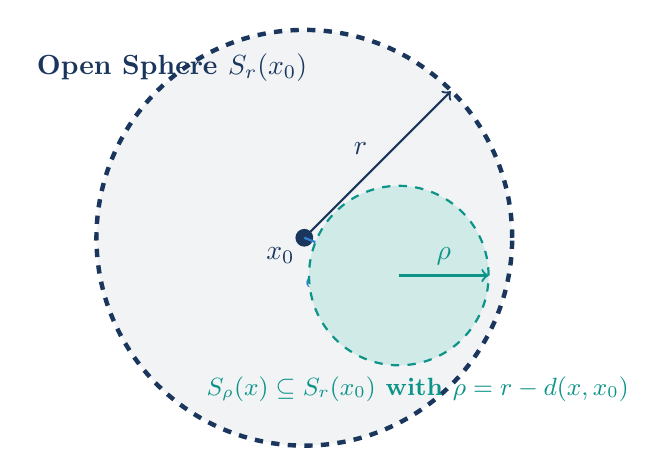
\begin{tikzpicture}[scale=1.2]
    % Outer open sphere S_r(x_0)
    \draw[dashed,ultra thick,primarynavy,fill=primarynavy!6] (0,0) circle (2.2cm);
    \filldraw[primarynavy] (0,0) circle (2.5pt) node[below left] {$x_0$};
    \draw[->,thick,primarynavy] (0,0) -- (1.55,1.55) node[midway,above left] {$r$};
    \node[primarynavy,font=\bfseries] at (-1.4,1.8) {Open Sphere $S_r(x_0)$};

    % Point x in S_r(x_0)
    \filldraw[secondaryteal] (1.0,-0.4) circle (2.5pt) node[below left] {$x$};
    \draw[thick,accentblue] (0,0) -- (1.0,-0.4) node[midway,below] {$d(x,x_0)$};

    % Inscribed open sphere S_rho(x)
    \draw[dashed,thick,secondaryteal,fill=secondaryteal!20] (1.0,-0.4) circle (0.95cm);
    \draw[->,thick,secondaryteal] (1.0,-0.4) -- (1.95,-0.4) node[midway,above] {$\rho$};
    \node[secondaryteal,font=\bfseries\small] at (1.2,-1.6) {$S_\rho(x) \subseteq S_r(x_0)$ with $\rho = r - d(x,x_0)$};
\end{tikzpicture}
\end{center}

\newpage

\begin{exbox}{Theorem 3: Arbitrary Union of Open Sets is Open}
\textbf{Theorem:} In a metric space $(X, d)$, the union of an arbitrary collection of open sets is an open set.

\textbf{Proof:}
\begin{enumerate}
    \item Let $\{G_\lambda \mid \lambda \in \Lambda\}$ be an arbitrary family of open sets in $(X, d)$.
    \item Let $G = \bigcup_{\lambda \in \Lambda} G_\lambda$.
    \item If $G = \emptyset$, then $G$ is open by Theorem 1.
    \item If $G \neq \emptyset$, let $x \in G$.
    \item By definition of the union, $x \in G_{\lambda_0}$ for some specific $\lambda_0 \in \Lambda$.
    \item Since $G_{\lambda_0}$ is open, there exists $r > 0$ such that $S_r(x) \subseteq G_{\lambda_0}$.
    \item Since $G_{\lambda_0} \subseteq \bigcup_{\lambda \in \Lambda} G_\lambda = G$, we have $S_r(x) \subseteq G$.
    \item Thus every point of $G$ is an interior point of $G$, proving that $G$ is \textbf{open}. \qed
\end{enumerate}
\end{exbox}

\begin{exbox}{Theorem 4: Finite Intersection of Open Sets is Open}
\textbf{Theorem:} In a metric space $(X, d)$, the intersection of a finite number of open sets is an open set.

\textbf{Proof:}
\begin{enumerate}
    \item Let $G_1, G_2, \dots, G_n$ be a finite collection of open sets in $(X, d)$.
    \item Let $G = \bigcap_{i=1}^n G_i$.
    \item If $G = \emptyset$, $G$ is open. If $G \neq \emptyset$, let $x \in G$.
    \item Then $x \in G_i$ for each $i \in \{1, 2, \dots, n\}$.
    \item Since each $G_i$ is open, there exist radii $r_1, r_2, \dots, r_n > 0$ such that $S_{r_i}(x) \subseteq G_i$ for each $i$.
    \item Define $r = \min \{r_1, r_2, \dots, r_n\}$. Since this is the minimum of finitely many positive numbers, $r > 0$.
    \item Then $S_r(x) \subseteq S_{r_i}(x) \subseteq G_i$ for all $i = 1, 2, \dots, n$.
    \item Consequently, $S_r(x) \subseteq \bigcap_{i=1}^n G_i = G$.
    \item Hence $x$ is an interior point of $G$, which proves $G$ is \textbf{open}. \qed
\end{enumerate}
\end{exbox}

\begin{formulabox}{Important Counterexample: Infinite Intersection of Open Sets May NOT be Open}
In $(\mathbb{R}, |\cdot|)$, consider the family of open intervals $G_n = \left(-\frac{1}{n}, \frac{1}{n}\right), \; n \in \mathbb{N}$.
\begin{equation}
    \bigcap_{n=1}^\infty G_n = \bigcap_{n=1}^\infty \left(-\frac{1}{n}, \frac{1}{n}\right) = \{0\}
\end{equation}
The singleton set $\{0\}$ is \textbf{closed} and \textbf{not open} in $\mathbb{R}$ because $\forall r > 0, S_r(0) = (-r, r) \not\subseteq \{0\}$.
\end{formulabox}

\subsection{Discrete Metric Space}

\begin{defbox}{Definition: Discrete Metric Space}
Let $X$ be any arbitrary non-empty set. The \textbf{discrete metric} on $X$ is defined as:
\begin{equation}
    d(x, y) = 0 \quad \text{if } x = y, \qquad \text{and} \qquad d(x, y) = 1 \quad \text{if } x \neq y
\end{equation}
\textbf{Key Topological Properties of Discrete Metric Spaces:}
\begin{itemize}
    \item For any point $x_0 \in X$ and radius $r \le 1$, $S_r(x_0) = \{x_0\}$. Thus, \textbf{every singleton set is an open ball}, and hence open.
    \item Since every subset is a union of singletons, \textbf{every subset in a discrete metric space is both open and closed (clopen)}.
\end{itemize}
\end{defbox}

\newpage

\section{Section 2: Closed Sets and Derived Sets}

\subsection{Closed Sets in Metric Spaces}

\begin{defbox}{Definition: Closed Set}
Let $(X, d)$ be a metric space. A subset $F \subseteq X$ is called a \textbf{closed set} if and only if its complement $F^c = X \setminus F$ is an open set in $(X, d)$.
\end{defbox}

\begin{exbox}{Examples of Closed Sets}
\begin{enumerate}
    \item \textbf{Singleton Sets in $(\mathbb{R}, |\cdot|)$:}
    For any $x \in \mathbb{R}$, the singleton $\{x\}$ is closed because its complement:
    $$\{x\}^c = (-\infty, x) \cup (x, \infty)$$
    is the union of two open intervals (open sets), hence open. Thus, \textbf{every singleton set in a metric space is closed}.
    
    \item \textbf{Closed Intervals in $(\mathbb{R}, |\cdot|)$:}
    The interval $[a, b]$ is closed because $[a, b]^c = (-\infty, a) \cup (b, \infty)$ is open.
\end{enumerate}
\end{exbox}

\subsection{Topological Properties of Closed Sets}

\begin{formulabox}{Duality Properties of Closed Sets}
\begin{enumerate}
    \item $\emptyset$ and $X$ are closed sets.
    \item The \textbf{arbitrary intersection} of closed sets is closed: $\left(\bigcap_{\lambda} F_\lambda\right)^c = \bigcup_{\lambda} F_\lambda^c$ (open).
    \item The \textbf{finite union} of closed sets is closed: $\left(\bigcup_{i=1}^n F_i\right)^c = \bigcap_{i=1}^n F_i^c$ (open).
\end{enumerate}
\end{formulabox}

\subsection{Limit Point Characterization of Closed Sets}

\begin{exbox}{Theorem: Closed Sets Contain All Their Limit Points}
\textbf{Theorem:} In a metric space $(X, d)$, a subset $F \subseteq X$ is closed if and only if $F$ contains all its limit points ($F' \subseteq F$).

\textbf{Proof:}
\begin{enumerate}
    \item \textbf{($\implies$) Necessary Condition:} Assume $F$ is closed $\implies F^c$ is open.
    \begin{itemize}
        \item If $F' = \emptyset$, then $F' \subseteq F$ holds trivially.
        \item If $F' \neq \emptyset$, let $p \in F'$. We must show $p \in F$.
        \item Suppose for contradiction that $p \notin F \implies p \in F^c$.
        \item Since $F^c$ is open, $\exists r > 0$ such that $S_r(p) \subseteq F^c = X \setminus F$.
        \item This implies $S_r(p) \cap F = \emptyset \implies (S_r(p) \setminus \{p\}) \cap F = \emptyset$.
        \item This contradicts the fact that $p$ is a limit point of $F$. Hence $p \in F$, so $F' \subseteq F$.
    \end{itemize}
    \item \textbf{($\impliedby$) Sufficient Condition:} Assume $F' \subseteq F$. We must show $F^c$ is open.
    \begin{itemize}
        \item Let $x \in F^c = X \setminus F$. Then $x \notin F \implies x \notin F'$ (since $F' \subseteq F$).
        \item Since $x$ is not a limit point of $F$, there exists $r > 0$ such that:
        $$(S_r(x) \setminus \{x\}) \cap F = \emptyset$$
        \item Since $x \notin F$, this gives $S_r(x) \cap F = \emptyset \implies S_r(x) \subseteq F^c$.
        \item Thus every point of $F^c$ is an interior point of $F^c$, so $F^c$ is open $\implies F$ is \textbf{closed}. \qed
    \end{itemize}
\end{enumerate}
\end{exbox}

\newpage

\subsection{Theorem: Every Derived Set is Closed}

\begin{exbox}{Theorem: The Derived Set $F'$ is Closed in $(X, d)$}
\textbf{Theorem:} Let $(X, d)$ be a metric space and $F \subseteq X$. Then the derived set $F'$ is a closed set in $(X, d)$.

\textbf{Proof:}
\begin{enumerate}
    \item We show that $(F')' \subseteq F'$, which proves $F'$ is closed.
    \item If $(F')' = \emptyset$, $(F')' \subseteq F'$ is trivial.
    \item Let $x \in (F')'$ (i.e., $x$ is a limit point of $F'$). We must prove $x \in F'$ (i.e., $x$ is a limit point of $F$).
    \item Let $S_r(x)$ be any open sphere centered at $x$ with radius $r > 0$.
    \item Since $x \in (F')'$, there exists a point $y_r \in F'$ distinct from $x$ with $y_r \in S_r(x)$.
    \item Thus $d(x, y_r) < r \implies \rho = r - d(x, y_r) > 0$.
    \item Consider the open sphere $S_\rho(y_r)$. By Theorem 2, $S_\rho(y_r) \subseteq S_r(x)$.
    \item Since $y_r \in F'$ ($y_r$ is a limit point of $F$), the sphere $S_\rho(y_r)$ contains a point $z_r \in F$ distinct from $y_r$:
    \begin{equation}
        z_r \in (S_\rho(y_r) \setminus \{y_r\}) \cap F
    \end{equation}
    \item Since $z_r \in S_\rho(y_r) \subseteq S_r(x)$, we have $z_r \in S_r(x)$ and $z_r \in F$.
    \item By choosing $\rho_1 = \min(\rho, d(x, y_r)) > 0$, we strictly ensure $z_r \neq x$.
    \item Therefore, $(S_r(x) \setminus \{x\}) \cap F \neq \emptyset$.
    \item This proves that $x$ is a limit point of $F \implies x \in F'$.
    \item Hence $(F')' \subseteq F'$, which establishes that $F'$ is a \textbf{closed set}. \qed
\end{enumerate}
\end{exbox}

\begin{center}
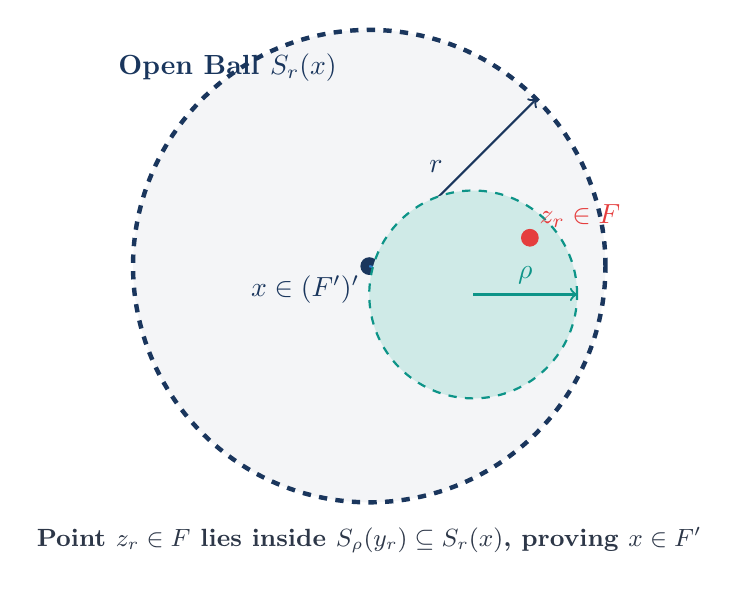
\begin{tikzpicture}[scale=1.2]
    % Outer open sphere S_r(x)
    \draw[dashed,ultra thick,primarynavy,fill=primarynavy!5] (0,0) circle (2.5cm);
    \filldraw[primarynavy] (0,0) circle (2.5pt) node[below left] {$x \in (F')'$};
    \draw[->,thick,primarynavy] (0,0) -- (1.77,1.77) node[midway,above left] {$r$};
    \node[primarynavy,font=\bfseries] at (-1.5,2.1) {Open Ball $S_r(x)$};

    % Limit point y_r in F'
    \filldraw[secondaryteal] (1.1,-0.3) circle (2.5pt) node[below=2pt] {$y_r \in F'$};
    \draw[thick,accentblue] (0,0) -- (1.1,-0.3) node[midway,below] {$d(x, y_r)$};

    % Inscribed sphere S_rho(y_r)
    \draw[dashed,thick,secondaryteal,fill=secondaryteal!20] (1.1,-0.3) circle (1.1cm);
    \draw[->,thick,secondaryteal] (1.1,-0.3) -- (2.2,-0.3) node[midway,above] {$\rho$};

    % Point z_r in F
    \filldraw[crimsonred] (1.7,0.3) circle (2.5pt) node[above right] {$z_r \in F$};
    
    \node[darkslate,font=\bfseries\small] at (0,-2.9) {Point $z_r \in F$ lies inside $S_\rho(y_r) \subseteq S_r(x)$, proving $x \in F'$};
\end{tikzpicture}
\end{center}

\newpage

\section{Section 3: Closure of a Set and Kuratowski Properties}

\subsection{Definition of Closure}

\begin{defbox}{Definition: Closure of a Set ($\overline{A}$)}
Let $(X, d)$ be a metric space and $A \subseteq X$. The \textbf{closure} of $A$, denoted by $\overline{A}$ or $\operatorname{Cl}(A)$, is defined as:
\begin{equation}
    \overline{A} = A \cup A'
\end{equation}
A point $x \in \overline{A}$ is called an \textbf{adherent point} of $A$ ($\forall r > 0, S_r(x) \cap A \neq \emptyset$).
\end{defbox}

\begin{formulabox}{Theorem: 7 Fundamental Properties of the Closure Operator}
Let $(X, d)$ be a metric space and $A, B \subseteq X$:
\begin{enumerate}
    \item[\textbf{(i)}] $\overline{A}$ is a \textbf{closed set} in $(X, d)$.
    \item[\textbf{(ii)}] \textbf{Monotonicity:} $A \subseteq B \implies \overline{A} \subseteq \overline{B}$.
    \item[\textbf{(iii)}] \textbf{Characterization:} $A$ is closed $\iff \overline{A} = A$.
    \item[\textbf{(iv)}] \textbf{Minimality:} $\overline{A}$ is the \textbf{smallest closed set} containing $A$.
    \item[\textbf{(v)}] \textbf{Finite Additivity:} $\overline{A \cup B} = \overline{A} \cup \overline{B}$.
    \item[\textbf{(vi)}] \textbf{Intersection Sub-additivity:} $\overline{A \cap B} \subseteq \overline{A} \cap \overline{B}$.
    \item[\textbf{(vii)}] \textbf{Idempotence:} $\overline{\overline{A}} = \overline{A}$.
\end{enumerate}
\end{formulabox}

\subsection{Complete Rigorous Proofs for Closure Theorems}

\begin{exbox}{Proof of Property (i): $\overline{A}$ is a Closed Set}
\textbf{To Prove:} $(\overline{A})^c$ is open.
\begin{enumerate}
    \item $(\overline{A})^c = (A \cup A')^c = A^c \cap (A')^c$.
    \item Let $x \in (\overline{A})^c = A^c \cap (A')^c \implies x \in A^c$ and $x \in (A')^c$.
    \item Since $x \notin A'$, $x$ is not a limit point of $A \implies \exists r_1 > 0$ such that $(S_{r_1}(x) \setminus \{x\}) \cap A = \emptyset$. Since $x \notin A$, $S_{r_1}(x) \cap A = \emptyset \implies S_{r_1}(x) \subseteq A^c$.
    \item Since $A'$ is closed, $(A')^c$ is open $\implies \exists r_2 > 0$ such that $S_{r_2}(x) \subseteq (A')^c$.
    \item Set $r^* = \min(r_1, r_2) > 0$. Then $S_{r^*}(x) \subseteq A^c \cap (A')^c = (\overline{A})^c$.
    \item Thus $(\overline{A})^c$ is open, so $\overline{A}$ is \textbf{closed}. \qed
\end{enumerate}
\end{exbox}

\begin{exbox}{Proof of Properties (ii), (iii), and (iv)}
\textbf{Proof of (ii):} Let $x \in A' \implies \forall r > 0, (S_r(x) \setminus \{x\}) \cap A \neq \emptyset$. Since $A \subseteq B$, $(S_r(x) \setminus \{x\}) \cap B \neq \emptyset \implies x \in B'$. Thus $A' \subseteq B'$. Hence $\overline{A} = A \cup A' \subseteq B \cup B' = \overline{B}$. \qed

\textbf{Proof of (iii):} $A$ is closed $\iff A' \subseteq A \iff \overline{A} = A \cup A' = A$. \qed

\textbf{Proof of (iv):} $\overline{A}$ is closed and $A \subseteq \overline{A}$. If $F$ is any closed set with $A \subseteq F$, then $\overline{A} \subseteq \overline{F} = F$. Hence $\overline{A} = \bigcap \{F \supseteq A \mid F \text{ is closed}\}$. \qed
\end{exbox}

\newpage

\begin{exbox}{Proof of Properties (v), (vi), and (vii)}
\textbf{Proof of (v) [$\overline{A \cup B} = \overline{A} \cup \overline{B}$]:}
\begin{enumerate}
    \item $A \subseteq A \cup B \implies \overline{A} \subseteq \overline{A \cup B}$, and $B \subseteq A \cup B \implies \overline{B} \subseteq \overline{A \cup B} \implies \overline{A} \cup \overline{B} \subseteq \overline{A \cup B}$.
    \item Also $A \subseteq \overline{A}, B \subseteq \overline{B} \implies A \cup B \subseteq \overline{A} \cup \overline{B}$. Since $\overline{A} \cup \overline{B}$ is closed, $\overline{A \cup B} \subseteq \overline{A} \cup \overline{B}$.
    \item Thus $\overline{A \cup B} = \overline{A} \cup \overline{B}$. \qed
\end{enumerate}

\textbf{Proof of (vi) [$\overline{A \cap B} \subseteq \overline{A} \cap \overline{B}$]:}
\begin{enumerate}
    \item $A \cap B \subseteq A \implies \overline{A \cap B} \subseteq \overline{A}$ and $A \cap B \subseteq B \implies \overline{A \cap B} \subseteq \overline{B} \implies \overline{A \cap B} \subseteq \overline{A} \cap \overline{B}$. \qed
    \item \textbf{Counterexample for Strict Inclusion:} For $A = (0, 1), B = (1, 2)$ in $\mathbb{R}$:
    $$\overline{A \cap B} = \overline{\emptyset} = \emptyset, \quad \text{while } \overline{A} \cap \overline{B} = [0, 1] \cap [1, 2] = \{1\} \neq \emptyset$$
\end{enumerate}

\textbf{Proof of (vii) [$\overline{\overline{A}} = \overline{A}$]:}
\begin{enumerate}
    \item Since $\overline{A}$ is closed (Property (i)), by Property (iii), $\overline{\overline{A}} = \overline{A}$. \qed
\end{enumerate}
\end{exbox}

\subsection{Perfect Sets}

\begin{defbox}{Definition: Perfect Set}
A subset $A \subseteq X$ is called a \textbf{perfect set} if and only if $A$ is closed and every point of $A$ is a limit point of $A$:
\begin{equation}
    \mathbf{A = A'}
\end{equation}
Equivalently, a perfect set is a closed set with \textbf{no isolated points}.
\end{defbox}

\begin{exbox}{Examples of Perfect Sets}
\begin{enumerate}
    \item Closed intervals $[a, b]$ in $(\mathbb{R}, |\cdot|)$ are perfect because $[a, b]' = [a, b]$.
    \item The whole Euclidean space $\mathbb{R}^n$ is perfect ($(\mathbb{R}^n)' = \mathbb{R}^n$).
    \item The Cantor Ternary Set $\mathcal{C} \subset [0, 1]$ is a compact, uncountably infinite perfect set of Lebesgue measure $0$.
    \item Singleton sets $\{x\}$ are closed but \textbf{not} perfect since $\{x\}' = \emptyset \neq \{x\}$.
\end{enumerate}
\end{exbox}

\begin{center}
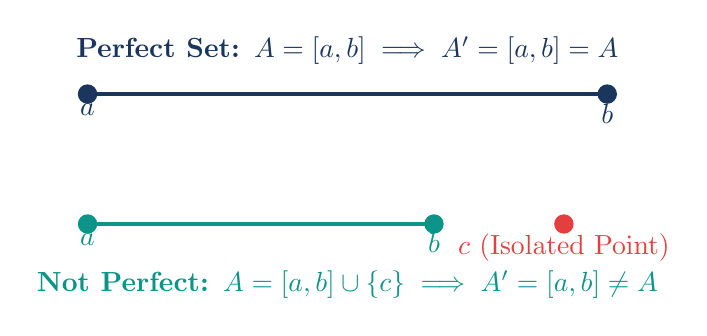
\begin{tikzpicture}[scale=1.1]
    % Closed interval [a, b] - perfect set
    \draw[ultra thick,primarynavy] (0,1.5) -- (6,1.5);
    \filldraw[primarynavy] (0,1.5) circle (3pt) node[below] {$a$};
    \filldraw[primarynavy] (6,1.5) circle (3pt) node[below] {$b$};
    \node[primarynavy,font=\bfseries] at (3,2.0) {Perfect Set: $A = [a, b] \implies A' = [a, b] = A$};
    
    % Non-perfect set: [a, b] U {c}
    \draw[ultra thick,secondaryteal] (0,0) -- (4,0);
    \filldraw[secondaryteal] (0,0) circle (3pt) node[below] {$a$};
    \filldraw[secondaryteal] (4,0) circle (3pt) node[below] {$b$};
    \filldraw[crimsonred] (5.5,0) circle (3pt) node[below] {$c$ (Isolated Point)};
    \node[secondaryteal,font=\bfseries] at (3,-0.7) {Not Perfect: $A = [a, b] \cup \{c\} \implies A' = [a, b] \neq A$};
\end{tikzpicture}
\end{center}

\newpage

\section{Section 4: The Interior Operator and Topological Boundary}

\subsection{Definition and Properties of Interior}

\begin{defbox}{Definition: Interior Operator ($A^\circ$ / $\operatorname{Int}(A)$)}
Let $(X, d)$ be a metric space and $A \subseteq X$. The \textbf{interior} of $A$ is:
\begin{equation}
    A^\circ = \operatorname{Int}(A) = \{ x \in A \mid \exists r > 0 \text{ such that } S_r(x) \subseteq A \}
\end{equation}
\end{defbox}

\begin{formulabox}{Theorem: Fundamental Properties of the Interior Operator}
\begin{enumerate}
    \item[\textbf{(i)}] $A^\circ \subseteq A$.
    \item[\textbf{(ii)}] $A^\circ$ is an \textbf{open set} in $(X, d)$.
    \item[\textbf{(iii)}] $A$ is open $\iff A^\circ = A$.
    \item[\textbf{(iv)}] If $B \subseteq A$ and $B$ is open, then $B \subseteq A^\circ$.
    \item[\textbf{(v)}] $A^\circ$ is the \textbf{largest open set} contained in $A$ ($A^\circ = \bigcup \{G \subseteq A \mid G \text{ is open}\}$).
    \item[\textbf{(vi)}] $(A \cap B)^\circ = A^\circ \cap B^\circ$ and $A^\circ \cup B^\circ \subseteq (A \cup B)^\circ$.
    \item[\textbf{(vii)}] $(A^\circ)^\circ = A^\circ$ (Idempotence).
\end{enumerate}
\end{formulabox}

\begin{exbox}{Proofs of Interior Theorems}
\textbf{Proof of (ii) [$A^\circ$ is Open]:}
\begin{enumerate}
    \item Let $x \in A^\circ \implies \exists r > 0$ such that $S_r(x) \subseteq A$.
    \item We show $S_r(x) \subseteq A^\circ$. Let $y \in S_r(x)$.
    \item By Theorem 2, $\exists \rho = r - d(x, y) > 0$ such that $S_\rho(y) \subseteq S_r(x) \subseteq A$.
    \item This shows $y$ is an interior point of $A \implies y \in A^\circ$.
    \item Thus $S_r(x) \subseteq A^\circ$, which proves $x$ is an interior point of $A^\circ$. Hence $A^\circ$ is open. \qed
\end{enumerate}

\textbf{Proof of (iii) [$A$ is open $\iff A^\circ = A$]:}
\begin{enumerate}
    \item If $A$ is open, every $x \in A$ is an interior point $\implies A \subseteq A^\circ \implies A^\circ = A$.
    \item Conversely, if $A = A^\circ$, since $A^\circ$ is open (by (ii)), $A$ is open. \qed
\end{enumerate}

\textbf{Proof of (iv) \& (v) [$A^\circ$ is largest open set in $A$]:}
\begin{enumerate}
    \item Let $B \subseteq A$ with $B$ open. Let $x \in B \implies \exists r > 0, S_r(x) \subseteq B \subseteq A \implies x \in A^\circ$.
    \item Hence $B \subseteq A^\circ$, so $A^\circ = \bigcup \{G \subseteq A \mid G \text{ is open}\}$. \qed
\end{enumerate}
\end{exbox}

\begin{formulabox}{Duality Relations and Topological Boundary}
\begin{equation}
    (A^c)^\circ = (\overline{A})^c, \qquad \overline{A^c} = (A^\circ)^c, \qquad \partial A = \operatorname{Bd}(A) = \overline{A} \setminus A^\circ = \overline{A} \cap \overline{A^c}
\end{equation}
\end{formulabox}

\newpage

\section{Section 5: Metric Subspaces and Relative Topologies}

\subsection{Definition of Metric Subspace}

\begin{defbox}{Definition: Metric Subspace $(Y, d_Y)$}
Let $(X, d)$ be a metric space, and let $Y$ be a non-empty subset of $X$.
\begin{itemize}
    \item Define $d_Y: Y \times Y \to \mathbb{R}$ by $d_Y(x, y) = d(x, y)$ for all $x, y \in Y$ (metric restriction).
    \item The pair $(Y, d_Y)$ is called a \textbf{Metric Subspace} of $(X, d)$.
    \item \textbf{Subspace Open Sphere:} For any $y_0 \in Y$ and $r > 0$:
    \begin{equation}
        S_r^Y(y_0) = \{ y \in Y \mid d_Y(y, y_0) < r \} = S_r^X(y_0) \cap Y
    \end{equation}
\end{itemize}
\end{defbox}

\begin{exbox}{Example: Relative Openness vs. Global Openness}
Let $(X, d) = (\mathbb{R}^2, d_2)$ and $Y = \{ (x, 0) \in \mathbb{R}^2 \mid x \in \mathbb{R} \}$ (the $x$-axis).
Let $E = (-1, 1) \times \{0\}$.
\begin{itemize}
    \item In the subspace $(Y, d_Y)$, $E = S_1^Y((0,0))$ is an open ball $\implies$ \textbf{$E$ is open relative to $Y$}.
    \item In the full space $\mathbb{R}^2$, every 2D open disk $S_r^{\mathbb{R}^2}((0,0))$ contains points with non-zero $y$-coordinates $\implies S_r^{\mathbb{R}^2}((0,0)) \not\subseteq E \implies$ \textbf{$E$ is NOT open in $\mathbb{R}^2$}.
\end{itemize}
\end{exbox}

\begin{center}
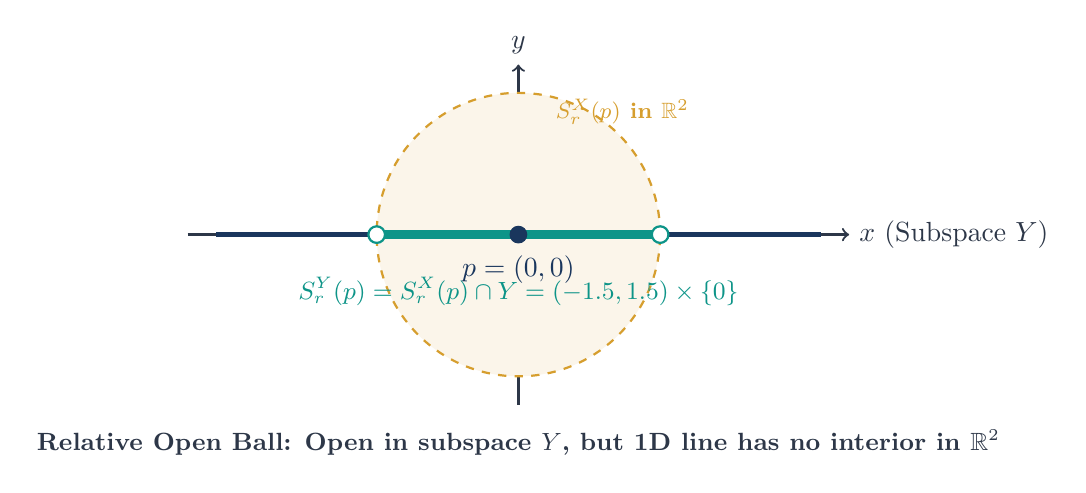
\begin{tikzpicture}[scale=1.2]
    % 2D Plane axes
    \draw[->,thick,darkslate] (-3.5,0) -- (3.5,0) node[right] {$x$ (Subspace $Y$)};
    \draw[->,thick,darkslate] (0,-1.8) -- (0,1.8) node[above] {$y$};
    
    % Subspace Y highlighted
    \draw[line width=2pt,primarynavy] (-3.2,0) -- (3.2,0);
    
    % 2D Ball in R^2: S_r^X(0)
    \draw[dashed,thick,warmgold,fill=warmgold!10] (0,0) circle (1.5cm);
    \node[warmgold,font=\bfseries\footnotesize] at (1.1,1.3) {$S_r^X(p)$ in $\mathbb{R}^2$};
    
    % Segment E = S_r^Y(p) = S_r^X(p) \cap Y
    \draw[line width=3.5pt,secondaryteal] (-1.5,0) -- (1.5,0);
    \draw[fill=white,draw=secondaryteal,thick] (-1.5,0) circle (2.5pt);
    \draw[fill=white,draw=secondaryteal,thick] (1.5,0) circle (2.5pt);
    \filldraw[primarynavy] (0,0) circle (2.5pt) node[below=4pt] {$p=(0,0)$};
    
    \node[secondaryteal,font=\bfseries\small] at (0,-0.6) {$S_r^Y(p) = S_r^X(p) \cap Y = (-1.5, 1.5) \times \{0\}$};
    \node[darkslate,font=\bfseries\small] at (0,-2.2) {Relative Open Ball: Open in subspace $Y$, but 1D line has no interior in $\mathbb{R}^2$};
\end{tikzpicture}
\end{center}

\newpage

\subsection{Fundamental Theorems on Subspace Topology}

\begin{exbox}{Theorem: Characterization of Relative Open Sets}
\textbf{Theorem:} Let $(Y, d)$ be a subspace of $(X, d)$. A subset $E \subseteq Y$ is \textbf{open relative to $Y$} if and only if there exists an open set $G \subseteq X$ such that:
\begin{equation}
    E = Y \cap G
\end{equation}

\textbf{Proof:}
\begin{enumerate}
    \item \textbf{($\implies$)} Assume $E$ is open in $Y$.
    \begin{itemize}
        \item For each $p \in E$, $\exists r_p > 0$ such that $S_{r_p}^Y(p) \subseteq E$.
        \item Note $S_{r_p}^Y(p) = S_{r_p}^X(p) \cap Y = V_p \cap Y$, where $V_p = S_{r_p}^X(p)$ is open in $X$.
        \item Let $G = \bigcup_{p \in E} V_p$. Since each $V_p$ is open in $X$, $G$ is an open set in $X$.
        \item Then $Y \cap G = Y \cap \left(\bigcup_{p \in E} V_p\right) = \bigcup_{p \in E} (Y \cap V_p) = \bigcup_{p \in E} S_{r_p}^Y(p) = E$.
        \item Thus $E = Y \cap G$ for the open set $G \subseteq X$.
    \end{itemize}
    \item \textbf{($\impliedby$)} Assume $E = Y \cap G$ for some open set $G \subseteq X$.
    \begin{itemize}
        \item Let $p \in E = Y \cap G \implies p \in Y$ and $p \in G$.
        \item Since $G$ is open in $X$, $\exists r > 0$ such that $S_r^X(p) \subseteq G$.
        \item Then $S_r^Y(p) = S_r^X(p) \cap Y \subseteq G \cap Y = E$.
        \item Thus $p$ is an interior point of $E$ in $Y$, so $E$ is \textbf{open relative to $Y$}. \qed
    \end{itemize}
\end{enumerate}
\end{exbox}

\begin{exbox}{Theorem: Characterization of Relative Closed Sets}
\textbf{Theorem:} Let $(Y, d)$ be a subspace of $(X, d)$. A subset $K \subseteq Y$ is \textbf{closed relative to $Y$} if and only if there exists a closed set $F \subseteq X$ such that:
\begin{equation}
    K = Y \cap F
\end{equation}

\textbf{Proof:}
\begin{enumerate}
    \item $K$ is closed in $Y \iff Y \setminus K$ is open in $Y$.
    \item By the Relative Open Set Theorem, $Y \setminus K = Y \cap G$ for some open set $G \subseteq X$.
    \item Taking complements in $Y$:
    \begin{equation}
        K = Y \setminus (Y \setminus K) = Y \setminus (Y \cap G) = Y \cap (X \setminus G) = Y \cap F
    \end{equation}
    where $F = X \setminus G = G^c$ is a \textbf{closed set in $X$}.
    \item Conversely, if $K = Y \cap F$ for closed $F \subseteq X$, then $Y \setminus K = Y \cap (X \setminus F) = Y \cap G$ (where $G = F^c$ is open), proving $K$ is closed in $Y$. \qed
\end{enumerate}
\end{exbox}

\begin{formulabox}{Corollaries: Inherited Openness and Closedness}
\begin{itemize}
    \item If $Y$ is \textbf{open} in $X$, then $E \subseteq Y$ is open in $Y \iff E$ is open in $X$.
    \item If $Y$ is \textbf{closed} in $X$, then $K \subseteq Y$ is closed in $Y \iff K$ is closed in $X$.
\end{itemize}
\end{formulabox}

\section{Section 6: Quick Revision Cheat Sheet on New Topics}

\begin{formulabox}{1. Open Sets, Spheres, and Derived Sets}
\begin{itemize}
    \item \textbf{Open Sphere $S_r(x_0)$:} $S_r(x_0) = \{x \in X \mid d(x, x_0) < r\}$.
    \item \textbf{Fundamental Ball Theorem:} Every open sphere $S_r(x_0)$ is an \textbf{open set} (radius $\rho = r - d(x, x_0) > 0$).
    \item \textbf{Open Set Properties:}
    \begin{itemize}
        \item $\emptyset$ and $X$ are open sets.
        \item Arbitrary union $\bigcup_{\lambda \in \Lambda} G_\lambda$ is open.
        \item Finite intersection $\bigcap_{i=1}^n G_i$ is open (Infinite intersection may fail: $\bigcap_{n=1}^\infty (-1/n, 1/n) = \{0\}$).
    \end{itemize}
    \item \textbf{Derived Set $A'$:} Set of all limit points of $A$. \textbf{Theorem:} $A'$ is always \textbf{closed} in $(X, d)$ ($(A')' \subseteq A'$).
\end{itemize}
\end{formulabox}

\begin{defbox}{2. Closed Sets, Closures, and Perfect Sets}
\begin{itemize}
    \item \textbf{Closed Set Characterization:} $F$ is closed $\iff F^c$ is open $\iff F' \subseteq F \iff \overline{F} = F$.
    \item \textbf{Closure Operator $\overline{A} = A \cup A'$:}
    \begin{itemize}
        \item $\overline{A}$ is closed; $A \subseteq B \implies \overline{A} \subseteq \overline{B}$; $\overline{\overline{A}} = \overline{A}$.
        \item $\overline{A}$ is the \textbf{smallest closed set} containing $A$.
        \item $\overline{A \cup B} = \overline{A} \cup \overline{B}$, and $\overline{A \cap B} \subseteq \overline{A} \cap \overline{B}$.
    \end{itemize}
    \item \textbf{Perfect Set:} $A$ is closed with no isolated points $\iff \mathbf{A = A'}$ (e.g., $[a, b]$, $\mathbb{R}^n$, Cantor Set $\mathcal{C}$).
\end{itemize}
\end{defbox}

\begin{formulabox}{3. Interior Operator, Boundary, and Metric Subspaces}
\begin{itemize}
    \item \textbf{Interior Operator $A^\circ = \operatorname{Int}(A)$:}
    \begin{itemize}
        \item $A^\circ \subseteq A$, and $A^\circ$ is an open set.
        \item $A$ is open $\iff A^\circ = A$.
        \item $A^\circ$ is the \textbf{largest open set} contained in $A$.
        \item $(A \cap B)^\circ = A^\circ \cap B^\circ$, and $(A^\circ)^\circ = A^\circ$.
    \end{itemize}
    \item \textbf{Duality \& Boundary:} $(A^c)^\circ = (\overline{A})^c$, $\overline{A^c} = (A^\circ)^c$, $\partial A = \overline{A} \setminus A^\circ = \overline{A} \cap \overline{A^c}$.
    \item \textbf{Metric Subspaces $(Y, d_Y)$ where $d_Y = d|_{Y \times Y}$:}
    \begin{itemize}
        \item Subspace Ball: $S_r^Y(y) = S_r^X(y) \cap Y$.
        \item \textbf{Relative Open Set Theorem:} $E \subseteq Y$ is open in $Y \iff \mathbf{E = Y \cap G}$ for some open set $G \subseteq X$.
        \item \textbf{Relative Closed Set Theorem:} $K \subseteq Y$ is closed in $Y \iff \mathbf{K = Y \cap F}$ for some closed set $F \subseteq X$.
    \end{itemize}
\end{itemize}
\end{formulabox}

\end{document}

